% arara: xelatex: {synctex: true}
% arara: indent: {overwrite: yes}
\documentclass[]{IMTexam}

\usepackage[enums,weirdsymbols]{IMTtikz}

\givecredits
\author{Isabella B.}
\USPN{11810773}
\date{}
\lecture{Física I} % disciplina
\lcode{4302111}
\hwtype{Resolução} % o que é
\examname{Lista 4} % prova

\begin{document}

\maketitle

\begin{quotation}
	\itshape ``To tell us that every species of things is endowed with an occult specific qua-
	lity by which it acts and produces manifest effects, is to tell us nothing. But
	to derive two or three general principles of motion from phenomena, and
	afterwards to tell us how the properties and actions of all corporeal things
	follow from those manifest principles, would be a very great step in Philosophy, though the causes of those principles were not yet discovered.''
	\par\raggedleft--- \textup{Newton}, Optics \textup{(citado por French)}
\end{quotation}

\begin{questions}

	\question
	Problemas em uma dimensão. Resolva as seguintes equações diferenciais sujeitas às condições iniciais dadas, isto é, encontre o valor da variável como função do tempo que satisfaça as condições iniciais. Os parâmetros $\omega_0, k, x_0 , y_0 , v_0 , a_0$  e $ C $ são constantes. Você verá em cálculo que a solução para essas equações é única!

	\begin{parts}
		\part \[ \dod{\theta}{t}=\omega_0 \, , \quad \theta\del{t=0}=\theta_0 \]

		\begin{solution}
			Vamos resolver essa equação diferencial por integração:
			\begin{align*}
				\int \dod{\theta}{t}\dif t & =\int \omega_0\dif t \\
				\intertext{como $ \dif\theta=\sbr{\od{\theta}{t}}\dif t $, temos}
				\int \dif\theta            & =\omega_0\,t+C_1     \\
				\theta(t)                  & =\omega_0\,t+C_1
			\end{align*}
			Como $ \theta(0)=C_1=\theta_0 $, temos:
			\[ \theta(t)=\omega_0\,t+\theta_0 \]
		\end{solution}

		\part \[ \dod[2]{x}{t}=k\, , \quad x\del{t=0}=x_0 \,\text{, e }\eval{\dod{x}{t}\del{t}}_{t=0}=v_0 \]

		\begin{solution}
			Fazendo idem ao item anterior:
			\begin{align*}
				\int \dod[2]{x}{t}\dif t   & =\int k\dif t \\
				\intertext{como $ \dif x=\sbr{\od{x}{t}}\dif t $, temos}
				\int \dod{}{t}\sbr{\dif x} & =k\,t+C_2     \\
				\dod{}{t}x(t)              & =k\,t+C_2
			\end{align*}
			Como $ \dod{x}{t}(t=0)=C_2=x_0 $, temos:
			\[ \dod{x}{t}(t)=k\,t+v_0 \]
			Integrando novamente, temos:
			\begin{align*}
				\int \dod{x}{t}\dif t & =\int k\,t+v_0 \dif t         \\
				\intertext{como $ \dif x=\sbr{\od{x}{t}}\dif t $, temos}
				\int \dif x           & =\dfrac{k}{2}t^{2}+v_0\,t+C_3 \\
				x(t)                  & =\dfrac{k}{2}t^{2}+v_0\,t+C_3
			\end{align*}
			Como $ x(t=0)=C_3=x_0 $, temos:
			\[ x(t)=\dfrac{k}{2}t^{2}+v_0\,t+x_0 \]
		\end{solution}

		\part \[ \dod[3]{y}{t}=C\, , \quad y\del{t=0}=y_0\,\text{, e }\eval{\dod{y}{t}\del{t}}_{t=0}=v_0\, , \quad\eval{\dod[2]{y}{t}\del{t}}_{t=0}=a_0 \]

		\begin{solution}
			Fazendo idem aos itens anteriores:
			\begin{align*}
				\int \dod[3]{y}{t}\dif t      & =\int C\dif t \\
				\intertext{como $ \dif y=\sbr{\od{y}{t}}\dif t $, temos}
				\int \dod[2]{}{t}\sbr{\dif y} & =C\,t+C_4     \\
				\dod[2]{}{t}y(t)              & =C\,t+C_4
			\end{align*}
			Como $ \dod[2]{y}{t}(t=0)=C_4=a_0 $, temos:
			\[ \dod[2]{y}{t}(t)=C\,t+a_0 \]
			Integrando novamente, temos:
			\begin{align*}
				\int \dod[2]{y}{t}\dif t   & =\int C\,t+a_0 \dif t         \\
				\intertext{como $ \dif y=\sbr{\od{y}{t}}\dif t $, temos}
				\int \dod{}{t}\sbr{\dif y} & =\dfrac{C}{2}t^{2}+a_0\,t+C_5 \\
				\dod{}{t}y(t)              & =\dfrac{C}{2}t^{2}+a_0\,t+C_5
			\end{align*}
			Como $ \od{y}{t}(t=0)=C_5=v_0 $, temos:
			\[ \dod{y}{t}(t)=\dfrac{C}{2}t^{2}+a_0\,t+v_0 \]
			Integrando novamente, temos:
			\begin{align*}
				\int \dod{y}{t}\dif t & =\int \dfrac{C}{2}t^{2}+a_0\,t+v_0 \dif t           \\
				\intertext{como $ \dif y=\sbr{\od{y}{t}}\dif t $, temos}
				\int \dif y           & =\dfrac{C}{6}t^{3}+\dfrac{a_0}{2}\,t^{2}+v_0\,t+C_6 \\
				y(t)                  & =\dfrac{C}{6}t^{3}+\dfrac{a_0}{2}\,t^{2}+v_0\,t+C_6
			\end{align*}
			Como $ y(t=0)=C_6=y_0 $, temos:
			\[ y(t)=\dfrac{C}{6}t^{3}+\dfrac{a_0}{2}\,t^{2}+v_0\,t+y_0 \]
		\end{solution}

	\end{parts}

	Note que você respondeu a quase todos os problemas matemáticos da cinemática do ensino médio. Encontre um exemplo para cada caso, de sistemas encontrados no seu dia a dia que possam ser modelados pelas equações nos casos acima. Caso tenha dificuldades com este problema você deve voltar a olhar o livro de cálculo.

	\question
	Duas naves da Federação no espaço interestelar, $ A $ e $ B $, encontram um objeto não identificado, que no referencial de $ A $ tem uma posição $\vec{r_A}(t)$, e $\vec{r_B}(t)$ no referencial de $ B $. As tripulações estão em contato e trocam informações. O oficial de Ciências a bordo de uma das naves faz a estimativa que a massa do objeto é $ M $. Também fazem medidas ao longo do tempo das posições do objeto, suficientes para estimar as acelerações do objeto em relação a cada uma das naves, a $ A $ e a $ B $, que se mostram constantes no tempo.

	\begin{parts}
		\part  Qual é o vetor de posição relativa $\vec{R_{AB}}$ da nave $ B $ com respeito à
		origem na nave $ A $?

		\begin{solution}

			\begin{multi}

				Pelo diagrama ao lado, podemos conferir que a transformação de Galileu correspondente é dada por
				\begin{equation}\label{eq:gTransform}
					\vec{r_A}=\vec{r_B}+\vec{R_{AB}}
				\end{equation}

				Portanto, $ \vec{R_{AB}}=\vec{r_A}-\vec{r_B} $.

				\nextcol
				\centering
				\begin{tikzpicture}
					\coordinate (Si) at (0,0);
					\draw[->] (Si)++(-0.5,0) -- +(2,0);
					\draw[->] (Si)++(0,-0.5) -- +(0,2);
					\node[below left] at (Si) {$ A $};

					\coordinate (Sd) at (3,2);
					\draw[->] (Sd)++(-0.5,0) -- +(2,0);
					\draw[->] (Sd)++(0,-0.5) -- +(0,2);
					\node[below right] at (Sd) {$ B $};

					\coordinate (obj) at (1,3);
					\draw[-Latex] (Si) -- node[above left] {$ \vec{r_A} $} (obj);
					\draw[-Latex] (Sd) -- node[above right] {$ \vec{r_B} $}(obj);
					\draw[-Latex] (Si) -- node[below right] {$ \vec{R_{AB}} $} (Sd);

					\filldraw (obj) circle (2pt) node[above] {Corpo};
				\end{tikzpicture}
			\end{multi}
		\end{solution}

		\part Suponha que $\vec{a_A} = \vec{a_B} = \vec{0}$. Esta informação é suficiente para dizer que o objeto não está acelerando e portanto é um referencial inercial? Antes de responder verifique se as naves estão com seus motores ligados.

		\begin{solution}
			Podemos conferir que três casos no problema:
			\begin{enumerate}[label=(\roman*)]
				\item Ambas as naves com os motores desligados:

				      Não é possível que o objeto esteja acelerando, pois, a partir de \ref{eq:gTransform}, temos:
				      \[ \dod[2]{}{t}\sbr{\vec{R_{AB}}}=\dod[2]{}{t}\sbr{\vec{r_A}-\vec{r_B}}\implies \vec{A_{AB}}=\vec{0} \]
				      portanto, as naves devem ser referenciais inerciais e, por consequência, o objeto também.

				\item Alguma das naves acelerando:

				      Esse caso é incoerente com a derivação anterior, pois a aceleração de uma nave em relação a outra deve ser nula, e isso implica que, se uma nave está acelerando, a outra também deve estar.

				\item Ambas naves acelerando:

				      Se ambas as naves estão acelerando, estamos num caso trivial, pois as naves não são referenciais inerciais, e se não medem aceleração do objeto, é porque ele também não o é.
			\end{enumerate}
		\end{solution}

		\part Suponha agora que $ \vec{a_A} = \vec{0}, \vec{a_B} \neq \vec{0} $. Verifique o estado de funcionamento dos motores.

		Há quatro casos: \begin{romanlistinline}[label=(\roman*)]
			\item ambos motores desligados, \item ambos ligados, \item $ A $ ligado e $ B $ desligado e \item $ A $ desligado e $ B $ ligado.
		\end{romanlistinline}

		Que podem concluir as tripulações em cada caso? Todos os casos são compatíveis com o que sabemos da mecânica?

		\begin{solution}
			Analisando caso a caso, temos:
			\begin{enumerate}[label=(\roman*)]
				\item Ambos motores desligados:

				      O caso em que ambos motores estão desligados e somente uma das naves percebe a aceleração é incoerente, pois, por \ref{eq:gTransform}:
				      \[ \dod[2]{}{t}\sbr{\vec{R_{AB}}}=\dod[2]{}{t}\sbr{\vec{r_A}-\vec{r_B}}\implies \vec{a_B}=\vec{a_A} \]
				      Portanto, a aceleração percebida por ambos referenciais deveria ser a mesma.

				\item Ambos motores ligados:

				      Com ambos motores ligados, o único caso possível é que $ B $ esteja se movendo com a mesma aceleração que o objeto, e $ A $, por estar com aceleração diferente, consegue medir a aceleração $\vec{a_A}$.

				      Outras situações desse caso são incoerentes.

				\item $ A $ ligado e $ B $ desligado:

				      Nesse caso, podemos concluir que o objeto realmente é um referencial inercial, e que $ A $ não o é.

				\item $ A $ desligado e $ B $ ligado:

				      O único caso possível, novamente, é que $ B $ se move com a mesma aceleração que o objeto, e como ambos não são referenciais inerciais, $ \vec{a_{A}} $ e $ \vec{a_{AB}} $ devem ser não-nulos.
			\end{enumerate}
		\end{solution}

		\part Agora $ \vec{a_A} \neq 0, \vec{a_B}\neq \vec{0} $. Qual é a força dos motores do objeto que cada tripulação pode calcular usando só a informação de sua aceleração com respeito ao objeto? Mostre que se $ \vec{a_A} \neq \vec{a_B} $ as tripulações chegam a conclusões diferentes. As leis da Física não são as mesmas nas duas naves? Calcule a diferença entre as forças estimadas pelas duas tripulações em função de medidas feitas do vetor de posição relativa $ \vec{R_{AB}} $. Note que se você não entende o significado de referencial inercial dificilmente pilotará uma das naves espaciais.

		\begin{solution}
			A tripulação, estimando a massa do objeto, pode calcular a força do motor do mesmo pela segunda lei de Newton. Porém, dependendo de seu estado, a aplicação da lei pode não ser válida.

			Analisando os casos, como antes, teremos:

			\begin{enumerate}[label=(\roman*)]
				\item Ambos motores desligados:

				      Se ambos motores estão desligados, as naves são referenciais inerciais, e a aceleração medida por cada uma deve ser a mesma, portanto, pela segunda lei de Newton, devem medir a mesma força.

				\item Ambos motores ligados:

				      Se ambos motores estão ligados, obviamente a aceleração das naves é diferente daquela do objeto. Se ambos possuem aceleração igual, vão concordar na medida da aceleração do objeto, e também no resultado da aplicação da segunda lei de Newton que, no entanto, estará errado, pois as naves não são referenciais inerciais nesse caso.

				      No caso de suas acelerações serem distintas, haverá disparidade entre as medidas na aceleração do objeto e, portanto, também haverá disparidade no cálculo da força.

				      Por \ref{eq:gTransform}, temos
				      \[ \dod[2]{}{t}\sbr{\vec{R_{AB}}}=\dod[2]{}{t}\sbr{\vec{r_A}-\vec{r_B}}\implies \vec{A_{AB}}=\vec{a_A}-\vec{a_B} \]

				      Desta forma a diferença entre as forças calculadas será proporcional à diferença entre as acelerações dois dois corpos.

				\item Alguma das naves com motor ligado:

				      Nesse caso, a nave que tem seus motores desligados conseguirá medir a aceleração verdadeira do objeto, e encontrará o resultado correto da força, e a outra não.

				      O fator de erro da nave que tem seus motores ligados será proporcional à aceleração $ \vec{A_{AB}} $, como no caso anterior.
			\end{enumerate}
		\end{solution}
	\end{parts}



	\question
	A teoria da relatividade começou com Galileu. Considere dois sistemas de referências e uma partícula cuja posição é descrita por $ (x,y,z,t) $ em um referencial e por $ (x_0, y_0, z_0, t_0) $ no outro. A transformação de Galileu é dada por
	\[ x'=x-v\,t\, ,\quad y'=y \, ,\quad z'=z \, ,\quad t'=t \]
	Considere movimento da partícula numa região do espaço onde o potencial só depende da posição e não da sua velocidade.

	\begin{parts}
		\part Mostre que a segunda lei de Newton tem a mesma forma nos dois referenciais descritos acima.

		\begin{solution}
			Assumindo que qualquer um dos referenciais é inercial (e, portanto, ambos são), podemos notar que, para as coordenadas $ y $ e $ z $, a transformação de Galileu é a própria coordenada, o que implica que os eixos $ y $ e $ z $ de ambos referenciais considerados se sobrepõem. Podemos, então, reduzir nossa análise ao eixo $ x $.

			Sendo $ x'=x-v\,t $, notamos que a velocidade do referencial $ (x_0,y_0,z_0,t_0) $ no eixo $ x $, em relação ao outro referencial, é igual à $ v $, e que é constante, portanto, a aceleração de um objeto qualquer medida em ambos referenciais deve ser a mesma.

			Pela segunda lei de Newton, a aceleração $ a $ de um objeto qualquer medida em qualquer um dos dois referenciais, será igual e terá valor $ F/m $, onde $ F $ é a força aplicada sobre o objeto, e $ m $ é sua massa.
		\end{solution}

		\part Uma pessoa, fixa no topo do mastro de um navio deixa cair uma pedra diretamente para baixo. Descreva as trajetórias vistas por uma pessoa parada no barco e outra parada no cais, vendo o barco passar a sua frente.

		\begin{solution}
			Como a pedra tem a mesma velocidade que o barco (desprezando qualquer atrito e a aceleração do barco), a pessoa fixa no mastro verá a pedra cair diretamente para baixo, e a pessoa no cais verá uma trajetória parabólica.



			\begin{multi}
				\centering
				\begin{tikzpicture}
					\begin{axis}[
							align =center,
							title={Altura por deslocamento\\ Referencial do mastro},
							every axis y label/.style={at={(current axis.north west)},above=0mm,xshift=0mm},
							every axis x label/.style={at={(current axis.right of origin)},anchor=west},
							axis lines=left,
							ylabel={$ y $},
							xlabel={$ x $},
							ticks=none,
							xmin=0,xmax=10,
							ymin=0,ymax=10,
						]
						\addplot[black,domain=1:9] {-x+10};
						%	\coordinate (A) at (axis cs:0,10);
					\end{axis}
				\end{tikzpicture}

				\nextcol

				\centering
				\begin{tikzpicture}
					\begin{axis}[
							align =center,
							title={Altura por deslocamento\\ Referencial do cais},
							every axis y label/.style={at={(current axis.north west)},above=0mm,xshift=0mm},
							every axis x label/.style={at={(current axis.right of origin)},anchor=west},
							axis lines=left,
							ylabel={$ y $},
							xlabel={$ x $},
							ticks=none,
							xmin=0,xmax=10,
							ymin=0,ymax=10,
						]
						\addplot[black,domain=1:9] {-x*x/10.125+9};
						%	\coordinate (A) at (axis cs:0,10);
					\end{axis}
				\end{tikzpicture}
			\end{multi}
		\end{solution}

		\part Uma pessoa, fixa no topo de uma ponte deixa cair uma pedra diretamente em cima de um navio que passa. Descreva as trajetórias vistas por uma pessoa parada no barco e outra parada na ponte.

		\begin{solution}
			Novamente, desprezando qualquer atrito, a pessoa fixa na ponte verá uma trajetória em linha reta para baixo, e a pessoa no barco verá a pedra fazer uma trajetória parabólica, se aproximando do barco conforme cai.

			\paragraph{Nota:}

			Os gráficos dos referenciais serão equivalentes aos do item anterior.
		\end{solution}

		\part Se a 2ª lei de Newton tem a mesma forma para os dois observadores porque a trajetória descrita não é a mesma?

		\begin{solution}
			A forma da segunda lei de Newton não diz respeito a mudanças de referencial por transformações de Galileu, e tais mudanças podem levar à alterações na trajetória vista por diferentes observadores.
		\end{solution}
	\end{parts}

	\question
	Um aluno distraído fez alguns comentários sobre mecânica. Discuta suas afirmações:

	\begin{parts}
		\part “A primeira Lei de Newton não passa de um caso particular da segunda Lei quando a força é zero”.

		\begin{solution}
			A primeira Lei de Newton é a definição de uma partícula isolada, e esta define um sistema inercial (em conjunto com um ``relógio''). A segunda Lei de Newton define os conceitos de aceleração e força, mas esses conceitos precisam da definição de um sistema inercial para funcionar, portanto a segunda Lei \textit{depende} da primeira.
		\end{solution}

		\part “A segunda Lei é a definição de força”.

		\begin{solution}
			A segunda Lei de Newton define a força como causa de uma aceleração, e a aceleração como efeito de uma força, e isso nos ajuda a identificar um sistema inercial, pois nele o movimento é uniforme, como descrito na primeira Lei.
		\end{solution}

		\part “A terceira Lei de Newton só se aplica para forças de contato”.

		\begin{solution}
			A gravidade é uma força de campo, e podemos notar sua presença em sistemas como Terra-Lua, onde as marés da Terra são influenciadas pela Lua, e esta tem uma órbita em torno da Terra. Esse efeito mútuo implica em um par ação reação.
		\end{solution}
	\end{parts}

	\question \label{ques:q5}
	Considere o movimento circular uniforme. Encontre a expressão para a aceleração centrípeta em função do raio e do módulo da velocidade. Mostre isso primeiro de forma geométrica e depois usando derivadas. Para essa parte, mostre que a forma paramétrica de um círculo é
	\[ x=r\cos\theta\, ,\quad y=r\sin\theta \]
	e portanto podemos escrever
	\[ \vec{r}=r\cos\theta\, \ehat{x}+r\sin\theta\, \ehat{y} \]
	onde $\ehat{x}$ e $\ehat{y}$ são versores (vetores de módulo 1) ao longo da direção crescente dos eixos $ x $ e $ y $, respectivamente.

	\begin{solution}

		\begin{multi}
			Seja a equação analítica do círculo
			\begin{equation}\label{eq:circAna}
				x^{2}+y^{2}=r^{2}
			\end{equation}
			onde $ r $ é seu raio. Dividindo ambos os lados por $ r^{2} $, temos
			\begin{align*}
				\del{\dfrac{x}{r}}^{2}+\del{\dfrac{y}{r}}^{2} & =1 \\
				\intertext{como as razões obedecem à relação fundamental da trigonometria, podemos introduzir um parâmetro $ \theta $}
				\del{\cos\theta}^{2}+\del{\sin\theta}^{2}     & =1
			\end{align*}

			\nextcol

			\centering
			\setmyunit{2cm}
			\begin{tikzpicture}
				\draw[->] (-1.5,0) -- (1.5,0) node[right] {$ x $} coordinate (x);
				\draw[->] (0,-1.5) -- (0,1.5) node[above] {$ y $};

				\coordinate (O) at (0,0);

				\draw (0,0) circle (1);
				\draw (0,0) -- (30:1) coordinate (r);
				\draw[decorate,decoration={brace,amplitude=3pt,raise=1pt,mirror}] (0,0) -- node[below=2pt,xshift=1pt] {$ x=r\cos\theta $} (r|-O) coordinate (xi);
				\draw[decorate,decoration={brace,amplitude=3pt,raise=1pt}] (0,0) -- node[left=2pt] {$ y=r\sin\theta $} (r-|O) coordinate (yi);

				\draw[dashed] (yi) -- (r) -- (xi);

				\pic[draw=black, angle radius=20pt,angle eccentricity=1,"$ \theta $" {xshift=5pt,yshift=1pt}] {angle=x--O--r};
			\end{tikzpicture}
		\end{multi}

		Interpretando o resultado geometricamente, temos a figura ao lado.

		Em notação vetorial, portanto, a vetor que descreve uma trajetória circular, a partir da origem, é
		\begin{equation}\label{eq:rvec}
			\vec{r}=r\cos\theta\, \ehat{x}+r\sin\theta\, \ehat{y}.
		\end{equation}

		Derivando $ \vec{r} $, encontramos a velocidade de uma partícula em movimento circular:
		\begin{align*}
			\dot{\vec{r}} & =\dod{}{t}\sbr{r\cos\theta\, \ehat{x}+r\sin\theta\, \ehat{y}}                                                                                 \\
			              & =\dot{r}\cos\theta\, \ehat{x}+r\dod{}{t}\sbr{\cos\theta\, \ehat{x}}+\dot{r}\sin\theta\, \ehat{y}+r\dod{}{t}\sbr{\sin\theta\, \ehat{y}}        \\
			\intertext{sendo o raio constante no movimento circular uniforme, $ \dot{r}=0 $ e $ \dot{\theta}=\omega $}
			              & =\cancelto{0}{\dot{r}}\del{\cos\theta\, \ehat{x}+\sin\theta\, \ehat{y}}+r\del{\omega\del{-\sin\theta}\, \ehat{x}+\omega\cos\theta\, \ehat{y}} \\
			\dot{\vec{r}} & =r\,\omega\del{-\sin\theta\, \ehat{x}+\cos\theta\, \ehat{y}}
		\end{align*}
		Tomando a segunda derivada do vetor $ \vec{r} $, temos:
		\begin{align*}
			\ddot{\vec{r}} & =\dod{}{t}\sbr{\dot{\vec{r}}}=\dod{}{t}\sbr{-r\,\omega\sin\theta\, \ehat{x}+r\,\omega\cos\theta\, \ehat{y}}                                                                  \\
			               & =-\dot{r}\,\omega\sin\theta\, \ehat{x}-r\dod{}{t}\sbr{\omega\sin\theta\, \ehat{x}}+\dot{r}\,\omega\cos\theta\, \ehat{y}+r\dod{}{t}\sbr{\omega\cos\theta\, \ehat{y}}          \\
			\intertext{sendo o raio constante no movimento circular uniforme, $ \dot{r}=0 $, e $ \dot{\omega}=\alpha $}
			               & =\cancelto{0}{\dot{r}}\del{-\omega\sin\theta\, \ehat{x}+\omega\cos\theta\, \ehat{y}}
			+r\del{-\alpha\sin\theta\, \ehat{x}-\omega\dod{}{t}\sbr{\sin\theta\, \ehat{x}}+
			\alpha\cos\theta\, \ehat{y}+\omega\dod{}{t}\sbr{\cos\theta\, \ehat{y}}}                                                                                                                       \\
			               & =r\del{\alpha\del{-\sin\theta\, \ehat{x}+\cos\theta\, \ehat{y}}+\omega\del{-\omega\cos\theta\, \ehat{x}+\omega\del{-\sin\theta}\, \ehat{y}}}                                 \\
			\ddot{\vec{r}} & =r\del{\alpha\del{-\sin\theta\, \ehat{x}+\cos\theta\, \ehat{y}}-\omega^{2}\del{\cos\theta\, \ehat{x}+\sin\theta\, \ehat{y}}}=r\,\alpha\,\dot{\vec{r}}-r\,\omega^{2}\,\vec{r}
		\end{align*}

		Tomando $ \vec{r}\cdot\dot{\vec{r}} $, temos
		\begin{align*}
			\vec{r}\cdot\dot{\vec{r}} & =\del{\cos\theta\,\ehat{x}}\cdot\del{-\sin\theta\, \ehat{x}}+\del{\sin\theta\, \ehat{y}}\cdot\del{\cos\theta\, \ehat{y}} \\
			                          & =-\cos\theta\cdot\sin\theta+\sin\theta\cdot\cos\theta=0
		\end{align*}
		portanto, os vetores são perpendiculares.

		Dessa fórmula, a componente $ r\,\alpha\,\dot{\vec{r}} $ de $ \ddot{\vec{r}} $ é uma aceleração tangencial, e $ -r\,\omega^{2}\,\vec{r} $ é uma aceleração apontando para o centro da trajetória, de módulo $ a_{cp}=r\,\omega^{2} $, a qual chamaremos de \textbf{aceleração centrípeta}.
	\end{solution}

	\clearpage

	\question
	Um martelo atinge um prego com velocidade $ v $, fazendo-o enterrar se de uma profundidade $\ell$ numa prancha de madeira. Mostre que a razão entre a força média exercida sobre o prego e o peso do martelo é igual a $h/\ell$, onde $ h $ é a altura de queda livre do martelo que o faria chegar ao solo com velocidade $ v $. Estime a ordem de grandeza dessa razão para valores típicos de $ v $ e $\ell$.

	\begin{solution}
		Sendo $ M $ a massa do martelo, e $ m $ a massa do prego, e $ v' $ a velocidade após a colisão do martelo com o prego, assumindo que não há forças externas no sistema, pela conservação de momento, temos que:
		\[ M\,v=(M+m)\,v'\implies v\approx v'  \]
		já que $ m\ll M $.

		Se o sistema martelo-prego realiza uma colisão perfeitamente elástica, e a massa do prego é desprezível, a força do prego sobre o martelo é aproximadamente igual à força do conjunto martelo-prego sobre o chão. Equacionando, temos
		\begin{equation}\label{eq:hammerFnailS}
			F_M=M\,a_m=(M+m)\,a'\implies a\approx a'.
		\end{equation}

		A aceleração do conjunto pode ser encontrada pela fórmula de Torricelli,
		\begin{equation}\label{eq:hammerNailAcc}
			0^{2}=v^{2}-2a'\,\ell\implies a=\dfrac{v^{2}}{2\ell}.
		\end{equation}

		Da mesma forma, podemos encontrar uma expressão para a aceleração da gravidade:
		\begin{equation}\label{eq:gravAcc}
			v^{2}=0^{2}+2g\,h\implies g=\dfrac{v^{2}}{2h}
		\end{equation}

		Tomando a razão desejada, temos
		\begin{align*}
			\dfrac{F_M}{P_M} & =\dfrac{M\,a'}{M\,g}                     \\
			\intertext{substituindo \ref{eq:hammerFnailS}, \ref{eq:hammerNailAcc} e \ref{eq:gravAcc}, temos}
			                 & \approx\dfrac{v^{2}/(2\ell)}{v^{2}/(2h)} \\
			\dfrac{F_M}{P_M} & =\dfrac{h}{\ell}
		\end{align*}

		\hfill\qedsymbol
	\end{solution}



	\question
	Uma criança desliza, para mergulhar dentro de uma piscina, do alto de um escorregador de \SI{3}{\meter} de comprimento e \ang{30} de inclinação com respeito à horizontal. A extremidade inferior do escorregador está \SI{3}{\meter} acima da água. A que distância horizontal dessa extremidade a criança mergulha na água?

	\clearpage

	\begin{solution}

		\begin{multi}
			Podemos dividir o movimento da criança em dois trechos:
			\begin{enumerate}[label=(\roman*)]
				\item corpo deslizando sobre plano inclinado;
				\item corpo em lançamento oblíquo.
			\end{enumerate}

			\paragraph{Nota:}
			A ilustração está fora de escala :(

			\nextcol
			\centering
			\begin{tikzpicture}
				\node[rotate=-30,anchor=south west] (C) at (0,-0.15) {
\includegraphics[scale=0.1]{child}};

				\coordinate (O) at (-30:4);

				\filldraw[white, draw=black] (60:0.25) -- (0,0) -- (O) -- +(60:0.25) -- cycle;

				\draw[dashed] (0,0) -- (60:-1) (O) -- +(60:-1);
				\draw[|<->|] ($ (0,0)+(60:-1)+(-30:-0.2pt) $) -- node[fill=white,inner sep=1pt,rotate=-30] {\SI{3}{\meter}} ($ (O)+(60:-1)+(-30:0.2pt) $);

				\draw[decorate, decoration={brace, mirror, raise=2pt,amplitude=5pt}] (O) ++(0,-2) -- node[below=5pt] {?} +(2,0);

				\draw[cyan!60] decorate[ragged border]{ (O) ++(-1,-2) coordinate (B) -- +(4,0)};

				\draw (B) -- ++(0,0.5) -- +(-1,0);
				\fill[pattern=north west lines] (B) -- ++(0,0.5) -- +(-1,0) -- cycle;

				\draw (-30:0.5) -- +(0,-1) (-30:0.5) ++(-30:0.5) -- +(0,-1);

				\fill[pattern=north west lines] ($ (-30:0.5)+(0,-1) $) -- (-30:0.5) -- ++(-30:0.5) -- +(0,-1) -- cycle;

				\coordinate (Or) at (0,0);
				\draw[dashed] (O) +(2,0) -- +(-1,0) coordinate (A);

				\draw[|<->|] ($ (O)+(2,0)+(0,0.3pt) $) -- node[inner sep=1pt,fill=white] {\SI{3}{\meter}} +(0,-2);

				\pic[draw=black, angle radius=20pt,angle eccentricity=1,"$ \ang{30} $" {xshift=-8pt,yshift=1pt}] {angle=Or--O--A};
			\end{tikzpicture}
		\end{multi}

		No primeiro trecho, assumindo que não haja atrito algum, a criança possui aceleração de $ g\sin\ang{30} $ na direção da superfície do escorregador, no sentido da descida e, portanto, ao final dos \SI{3}{\meter}, possui velocidade $ v_e=\sqrt{2\cdot3g\sin\ang{30}}=\sqrt{3g} $ (por Torricelli).

		No segundo trecho do movimento a criança é lançada do escorregador com velocidades iniciais $ v_{0x}=v_e\cos\ang{30} $ e $ v_{0y}=v_e\sin\ang{30} $ nos eixos $ x $ e $ y $, respectivamente, adotando o sentido para baixo como positivo no eixo $ y $.

		Analisando o tempo necessário para atingir a superfície da água, temos
		\[ 0=3-v_{0y}\,t-\dfrac{g}{2}\,t^{2}\implies -3+\sqrt{3g}\dfrac{t}{2}+\dfrac{g}{2}\,t^{2}=0  \]
		sendo o ponto médio da parábola $ m=-\sqrt{3g}/(2g) $, e a distância entre as raízes $ d=\sqrt{m^{2}+6/g} $, temos a raiz positiva
		\[ t=-\dfrac{\sqrt{3g}}{2g}+\sqrt{\del{\dfrac{\sqrt{3g}}{2g}}^{2}+\dfrac{6}{g}}\implies t=\dfrac{\sqrt{3g}}{g} \]
		portanto, a criança percorre
		\[ d=v_{0x}\,t=\sqrt{3g}\cos\ang{30}\del{\sqrt{3g}}/g=3g\sqrt{3}/(2g)\approx\SI{2.6}{\meter} \] a partir da extremidade, até atingir a água.
	\end{solution}



	\question
	O dispositivo da Fig. \ref{fig:fig1} gira em torno do eixo vertical com a velocidade angular $\omega$.

	\begin{figure}[H]
		\centering
		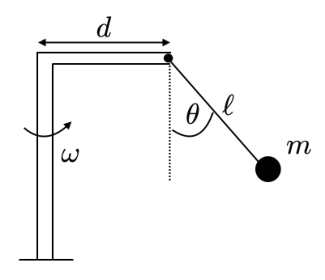
\includegraphics[width=0.35\linewidth]{screenshot001}
		\caption{Dispositivo girante}
		\label{fig:fig1}
	\end{figure}

	\begin{parts}
		\part Qual deve ser o valor de $\omega$ para que o fio de comprimento $\ell$ com a bolinha suspensa de massa $ m $ faça um ângulo $ \theta $ com a vertical?

		\begin{solution}
			Como o movimento da massa $ m $ é rotacional, ela estará sujeita a uma aceleração centrípeta, numa trajetória de raio $ r=d+\ell\sin\theta $. Como a velocidade angular $ \omega $ é constante, a massa está em equilíbrio, e o somatório das forças deve ser zero.

			Sendo $ \vec{P} $ a força peso e $ \vec{T} $ a tensão do fio as únicas forças que atuam sobre a massa $ m $, o módulo da componente vertical da tensão $ T_y=T\cos\theta $ deve igualar o módulo do peso $ P=m\,g $, portanto:
			\begin{equation}\label{eq:Tmg}
				T_y=P\implies T\cos\theta=m\,g\implies T=\dfrac{m\,g}{\cos\theta}
			\end{equation}

			Como a componente horizontal da tensão $ T_x=T\sin\theta $ será nossa força centrípeta $ F_c $ --- que segura a massa na trajetória circular --- pela segunda lei de Newton, temos
			\begin{equation}\label{eq:fcNewton}
				F_c=T_x=m\,a_{cp}\implies a_{cp}=\dfrac{T\sin\theta}{m}
			\end{equation}

			Tomando $ a_{cp}=\omega^{2}\,r $ (da questão \ref{ques:q5}), temos
			\begin{align}
				\omega^{2}\,r & =\dfrac{T\sin\theta}{m}\nonumber                                                             \\
				\intertext{substitiondo \ref{eq:Tmg}, temos}
				|\omega|      & =\sqrt{\dfrac{m\,g}{r\cos\theta}\dfrac{\sin\theta}{m}}\nonumber                              \\
				\omega        & =\sqrt{\dfrac{g}{r}\tan\theta}\quad\text{assumindo $ \omega\geqslant0 $.}\label{eq:omegaRes}
			\end{align}
		\end{solution}

		\part Qual a tensão $ T $ no fio nessa situação?

		\begin{solution}
			Tomando \ref{eq:fcNewton}, temos:
			\begin{align*}
				T & =\dfrac{m}{\sin\theta}a_{cp}                                                                            \\
				\intertext{como $ a_{cp}=\omega^{2}\,r $,}
				  & =\dfrac{m}{\sin\theta}\omega^{2}\,r                                                                     \\
				\intertext{substituindo \ref{eq:omegaRes}}
				  & =\dfrac{m}{\sin\theta}\del{\sqrt{\dfrac{g}{r}\tan\theta}}^{2}r                                          \\
				  & =\dfrac{m}{\cancel{\sin\theta}}\dfrac{\cancel{\sin\theta}}{\cos\theta}\dfrac{g}{\cancel{r}}\,\cancel{r} \\
				T & =\dfrac{m\,g}{\cos\theta}
			\end{align*}
		\end{solution}

	\end{parts}

	\question
	Um feixe de prótons movendo-se ao longo de uma direção tomada como eixo $ Ox $, com velocidade de \SI{1e6}{\meter\per\second}, penetra numa região onde existe um campo magnético uniforme de intensidade 100 gauss, dirigido ao longo do eixo $ Oz $. Calcule a deflexão do feixe na direção $ y $, após penetrar uma distância de \SI{50}{\centi\meter} ao longo da direção $ x $ na região onde existe o campo magnético.

	\begin{solution}

		\correctspacing
		\begin{multi}
			Sendo a força magnética $ \vec{F_m} $ sobre uma partícula igual a sua carga vezes o produto vetorial da velocidade $ \vec{v} $ com o vetor campo magnético $ \vec{B} $, temos que a força sempre será perpendicular à velocidade da partícula, o que provoca um movimento circular. Considerando que cada próton se move pela mesma trajetória, podemos analisar o movimento de um único próton e generalizar o resultado.

			\nextcol

			\centering
			\begin{tikzpicture}[scale=1.5]
				\newcommand{\magFs}{1.5}
				\foreach \i in {-1,0,1}{
						\foreach \j in {-1,0,1}{
								\draw[red] ($ (\i,\j)+(4,0.6)+(8pt,0) $) circle (4pt);
								\draw[red] ($ (\i,\j)+(4,0.6)+(8pt,0) $) ++(\magFs pt,\magFs pt) -- ++(-2*\magFs pt,-2*\magFs pt) ++(0,2*\magFs pt) -- +(2*\magFs pt,-2*\magFs pt);
							}
					}
				\node[red] at ($ (3,1)+(8pt,3pt) $) {$ \vec{B} $};

				\draw[densely dotted] (2,0) -- ++(1,0) arc (-90:-28.8:2.91);
				\draw[-Latex] (3,2.91) ++(-55:2.91) -- node[above right] {$ \vec{F_m} $} +(-55:-1);
				\draw[-Latex] (3,2.91) ++(-55:2.91) -- +(35:1) node[right] {$ \vec{v} $};

				\begin{scope}[shift={(6.5,0)}]
					\draw[->] (xyz cs:x=-.8) -- (xyz cs:x=.8) node[right] {$x$};
					\draw[->] (xyz cs:y=-.8) -- (xyz cs:y=.8) node[above] {$y$};
					\draw[->] (xyz cs:z=.8) -- (xyz cs:z=-.8) node[right] {$z$};
				\end{scope}
			\end{tikzpicture}
		\end{multi}

		Pela segunda lei de Newton, temos
		\begin{align*}
			|\vec{F_m}|=|q\,\vec{v}\times\vec{B}| & =m\,a_{cp}                                                                                      \\
			m\,\omega^{2}\,r                      & =q\,v\,B\sin\theta                                                                              \\
			\intertext{como $ \omega=v/r $, e um próton tem massa $ m=m_p $ e carga $ q=q_p $, temos}
			r                                     & =\dfrac{m_p\,v}{q_p\,B}=\dfrac{\num{1e6}}{\num{0.01}}\dfrac{m_p}{q_p}=\num{1e8}\dfrac{m_p}{q_p}
		\end{align*}

		Sendo \[ \omega=\dot{\theta}\implies \theta(t)=\omega\,t+\omega_0 \]
		assumindo $ \omega_0=0 $, temos $ \theta(t)=\omega\,t $, onde $ \omega=v/r $.

		Sendo o deslocamento no eixo $ x $ igual à $ \num{0.5}=r\cos\theta\implies\omega\,t=\arccos\del{\num{0.5}/r} $, pela questão \ref{ques:q5}, a equação da posição da partícula em movimento circular uniforme pode ser escrita como:
		\[ \vec{r}(t)=r\cos\omega\,t\,\ihat+r\sin\omega\,t\,\jhat. \]

		Analisando somente a componente na direção do eixo $ y $, temos, para $ \omega\,t=\arccos\del{\num{0.5}/r} $ a deflexão de
		\begin{align*}
			y_d & =r\sin\del{\arccos\del{\dfrac{\num{0.5}}{r}}}                                                                                         \\
			    & =r\sqrt{1-\cos^{2}\del{\arccos\del{\dfrac{\num{0.5}}{r}}}}                                                                            \\
			    & =r\sqrt{1-\del{\dfrac{\num{0.5}}{r}}^{2}}                                                                                             \\
			    & =\sqrt{r^{2}-\num{0.5}^{2}}                                                                                                           \\
			\intertext{substituindo $ r=\num{1e8}\dfrac{m_p}{q_p} $, para $ m_p=\SI{1.67e-27}{\kilogram} $ e $ q_p=\SI{1.60e-19}{\coulomb} $, temos}
			    & =\sqrt{\del{\num{1e8}\dfrac{\num{1.67e-27}}{\num{1.60e-19}}}^{2}-\num{0.5}^{2}}=\sqrt{\num{1.04}^{2}-\num{0.5}^{2}}=\SI{0.91}{\meter}
		\end{align*}


		%		Dessa forma, se um próton percorre \SI{50}{\centi\meter} em $ t=\num{0.5}/\num{1e6}=\SI{5.0e-7}{\second} $.
	\end{solution}

	\clearpage

	\question
	Uma partícula de massa $ m $ movendo ao longo de uma linha reta sente uma força de retardamento (uma força que sempre opõe ao movimento) $ F=b\,\mathrm{e}^{\alpha\,v} $, onde $ b $ e $\alpha$ são constantes e $ v $ é a velocidade. Em $ t = 0 $ a velocidade da partícula é $ v_0 $, encontre a velocidade da partícula em tempos posteriores.

	\begin{solution}
		Pela segunda lei de Newton,
		\begin{align*}
			F=b\,\mathrm{e}^{\alpha\,v}                 & =m\,\dod{v}{t}                                               \\
			\mathrm{e}^{-\alpha\,v}\dod{v}{t}           & =\dfrac{b}{m}                                                \\
			\intertext{integrando com respeito ao tempo, temos}
			\int\mathrm{e}^{-\alpha\,v}\dod{v}{t}\dif t & =\int\dfrac{b}{m}\dif t                                      \\
			\intertext{fazendo $ u=-\alpha\,v\implies \dif u=-\alpha\dif v $ e $ \dif v=\sbr{\od{v}{t}}\dif t $, temos}
			-\dfrac{1}{\alpha}\int\mathrm{e}^{u}\dif u  & =\dfrac{b}{m}\,t+C                                           \\
			\mathrm{e}^{-\alpha\,v(t)}                  & =-\alpha\del{\dfrac{b}{m}\,t+C}                              \\
			v(t)                                        & =-\dfrac{1}{\alpha}\ln{\del{-\alpha\del{\dfrac{b}{m}\,t+C}}}
		\end{align*}
		como $ v(t=0)=v_0 $, temos
		\[ v_0=-\dfrac{1}{\alpha}\ln -\alpha\,C\implies C=-\dfrac{1}{\alpha}\mathrm{e}^{-\alpha\,v_0} \]
		portanto
		\begin{align*}
			v(t) & =-\dfrac{1}{\alpha}\ln{\del{\mathrm{e}^{-\alpha\,v_0}-\alpha\dfrac{b}{m}\,t}}
		\end{align*}
	\end{solution}

\end{questions}
\end{document}
